\chapter[\hermes: A hybrid integrator]{\hermes: a hybrid integrator for simulating close encounters and planetesimal migration}
\label{chap:Hermes}

\section{Chapter Overview}
	\begin{center}
	\begin{minipage}[c]{4.75in}
	The work and figures from this Chapter has been done in collaboration with my supervisor Hanno Rein and Center for Planetary Science postdoc Daniel Tamayo. 
	A publication is currently in preparation. 
	\vspace{2em}
	\end{minipage}
	\end{center}

We present \hermes, a new hybrid integration scheme for long-term simulations of planetary systems undergoing close encounters or planetesimal-driven migration. 
Particles are integrated using \whfast, a fast and accurate symplectic integrator, unless a close encounter occurs.
During a close encounter, a subset of particles is integrated with the high-order integrator \ias, while the rest of the particles continue to be integrated with \whfast.
We created an adaptive routine for optimizing the close encounter boundary to help maintain accuracy whilst close encounters are occurring.

Like most hybrid integrators, the switching between integrators leads to an additional, finite energy error above the standard oscillatory energy error arising from symplectic integration.
\hermes takes a more direct approach when switching between integrators than previous schemes in the literature, allowing us to analytically estimate the numerical error of our algorithm. 
Since \whfast is symplectic, \ias is accurate to machine precision and both of them are unbiased, the energy error grows sub-linearly with time under the assumption that either impact parameters are randomly distributed or close encounters are rare.

We find that \hermes provides a good balance between speed and accuracy, neither achieved by the individual symplectic or non-symplectic integrators alone.
In this Chapter, we describe the details of implementation, accuracy and performance, as well as its incorporation within the larger framework of the $N$-body package \reb. 

\section{Introduction}
\label{sec:intro}
Over the last 25 years scientists have made considerable progress integrating $N$ gravitationally interacting particles (an $N$-body system) using computational techniques. 
The most widely used integrator today for solving Solar System type problems is the Wisdom-Holman integrator \citep[hereafter WH]{Wisdom1991}, which decomposes the system's Hamiltonian, $H$, into a Keplerian and an interaction component, $H_K$ and $H_I$. 
Symplectic integrators which split the Hamiltonian in this way are known as mixed-variable symplectic integrators \citep{Wisdom1991, Saha1992}.
The system is then evolved in a second-order leapfrog manner, taking the form of $K($dt$/2) I($dt$) K($dt$/2)$, where $K$ represents evolution under $H_K$, $I$ represents evolution under $H_I$, and $dt$ is the timestep.
Although higher-order algorithms are possible \citep[e.g.][]{Yoshida1990}, the second-order WH method is an ideal balance of speed and accuracy, since the marginal increase in accuracy of higher-order methods comes at the cost of significant additional calculation. 
The evolution under the interaction Hamiltonian is trivial to solve exactly in Cartesian coordinates, whereas the evolution under the Keplerian Hamiltonian is easy to solve exactly using orbital elements. 
This algorithm therefore converts between the two coordinate systems each timestep.

Since the WH scheme breaks the evolution into operators that both derive from Hamiltonians, the algorithm is symplectic (for a review on symplectic algorithms see \citet{Yoshida1993}).
This implies that the numerical solution conserves quantities closely related to the integrals of motion, such as the total energy. 
In practice these integrals of motion are not constant, but oscillate in a bounded manner.
The relative energy error scales as $O(\epsilon dt^2)$ if the magnitude of $H_I$ remains $O(\epsilon)$ smaller than $H_K$, where $\epsilon \ll 1$ \citep{Saha1994}. 
For distant particles in non-overlapping orbits $\epsilon$ is typically much less than unity.
This is one motivation for splitting $H$ into $H_K$ and $H_I$, as it allows for longer timesteps (and thus shorter integration times) than conventional integration schemes. 
However, during close encounters, $H_I$ becomes comparable to or larger than $H_K$ causing $\epsilon$, and thus the energy error, to grow substantially. 
Therefore, despite their brief duration, close encounters typically dictate an unacceptably short timestep for the entire simulation. 
Note that it is not possible to dynamically change the timestep in the standard WH integrator as it would break time symmetry and symplecticity\footnote{If one can make the timestep choice independent of the current state, for example by using a predefined sequence of timesteps, then the integrator remains symplectic.}.

For very high accuracy integrations (with relative errors of order the machine precision), non-symplectic integrators are as good and as fast as or faster than symplectic integrators \citep{Rein2015a}.
But in most integrations, medium to low accuracy is enough to capture the qualitative evolution of a system. 
In such a case a symplectic integrator provides an advantage as the timestep can be large while keeping the numerical errors bounded.
This advantage of symplectic integrators, together with the common need to accurately resolve close encounters motivates the development of hybrid integrators that can make use of both symplectic and non-symplectic integrators.

Several hybrid integrators that make use of a (modified) WH integrator have been developed. 
The two most popular ones are \symba \citep{Duncan1998} and the hybrid integrator from the \mercury package \citep[hereafter referred to as \mercury]{Chambers1999}.

\symba decomposes the interaction potential into a series of shells around each body and uses progressively smaller timesteps for each shell to increase time resolution.
If the particles are well separated, there is only one contributing shell to the interaction term and the integrator is effectively WH.
During a close encounter the inner shells contribute to the integration using smaller timesteps to resolve the encounter.

\mercury handles close encounters by using a smooth changeover function to transfer large terms from $H_I$ to $H_K$. 
When particles are distant, interactive forces between particles are small and evaluated during $H_I$. 
When particles are close, interactive forces become large and are transferred to $H_K$, thus keeping $H_I$ small. 
This makes $H_K$ a three body problem (central body plus two particles undergoing a close encounter) which cannot be solved analytically but is straightforward to integrate numerically to high precision using a Bulirsch-Stoer routine \citep{BS1988}. 
 
In this Chapter we present a new integration method, \hermes, which borrows ideas from the integrators mentioned above, but takes a more direct approach to handling close encounters.
It combines two existing integrators, \whfast \citep{Rein2015b} 
 which is a fast and unbiased implementation of the WH method, and the high-order \ias integrator \citep{Rein2015a}. 
\hermes has been seamlessly incorporated into \reb \citep{Rein2012}, adding further flexibility to the modular $N$-body package. 

The outline for the Chapter is as follows: Section~\ref{sec:Methods} describes the algorithm for \hermes, Section~\ref{sec:Error} characterizes error, Section~\ref{sec:Examples} shows standard tests of \hermes as well as a comparison to \symba and \mercury, and we conclude in Section~\ref{sec:Conclusion}.

%%%%%%%%%%%%%%%%%%%%%%%%%%%%%%%%%%%%%%%%%%%%%%%%%%%
%%%%%%%%%%%%%%%%%%%%%%%%%%%%%%%%%%%%%%%%%%%%%%%%%%%
\section{Methods}
\label{sec:Methods}

%%%%%%%%%%%%%%%%%%%%%%%%%%%%%%%%%%%%%%%%%%%%%%%%%%%
\subsection{Particle Classification}
First we define the three different types of particles handled by \hermes: active particles, semi-active particles and test particles. 
Active particles can gravitationally affect all other types of particles, and are typically stars or planets.
Semi-active particles can affect active particles only (not other semi-active particles), and are typically asteroids, planetesimals, and other smaller objects.
Test particles are only affected by active particles and cannot affect any other particle, and are typically dust grains, rocks, small asteroids or spacecrafts. 
Figure~\ref{fig:bodies} summarizes these interactions, where arrows represent directions of gravitational influence.

\begin{figure}
\centerline{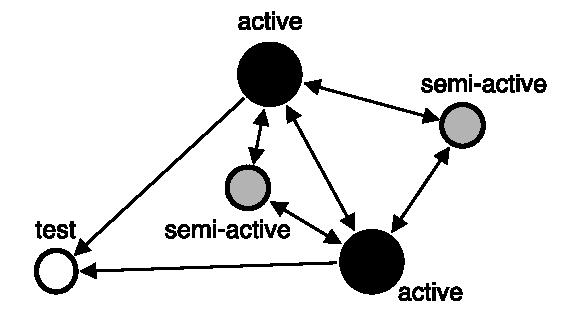
\includegraphics[scale=0.6]{chap4/images/bodies.pdf}}
\caption{A diagram illustrating how different particle types (active, semi-active, test) affect each other. Arrows indicate directions of gravitational influence.
 }
\label{fig:bodies}
\end{figure}

%%%%%%%%%%%%%%%%%%%%%%%%%%%%%%%%%%%%%%%%%%%%%%%%%%%
%\subsection{Heliocentric version of \whfast}
%\memoas{If cant get WHDS to work, remove this paragraph}
%The original \whfast algorithm described in  \cite{Rein2015b} was implemented in Jacobi coordinates.
%Jacobi coordinates lead to a better precision compared to heliocentric coordinates if orbits are well separated and do not cross each other. 
%If close encounter occur, then heliocentric coordinates can help improve the integrator's accuracy.
%For that reason we implemented a heliocentric version of \whfast in \reb.
%We call it \whfasthelio.
%We use it as the symplectic integrator in \hermes but note that \whfasthelio can also be used by itself. 
%We choose the specific splitting of the Hamiltonian by \cite{Duncan1998} and \cite{Chambers1999}.
%For a discussion on the different splittings, their advantages and disadvantages, see \cite{Wisdom2006}. 
%For the remainder of this Chapter we will refer to \whfasthelio simply as \whfast as both integrators use the same Kepler solver.

%%%%%%%%%%%%%%%%%%%%%%%%%%%%%%%%%%%%%%%%%%%%%%%%%%%
\subsection{Algorithm}
\label{sec:Alg}
The \hermes integrator is composed of two parts, a \textit{global} simulation which contains all particles, and a \textit{mini} simulation which contains all active particles plus any semi-active or test particles involved in a close encounter.
The global simulation is integrated using \whfast, while the mini simulation is integrated using \ias. 
We first outline the overall algorithm for one timestep\footnote{We refer to the timestep that \whfast takes as $dt$. The \ias integrator chooses its own timestep which is typically smaller than $dt$.}  of length $dt$ and then describe the individual steps in more detail.

To evolve the system for a single timestep \hermes performs the following steps:
\begin{enumerate}
\item \label{step1} \textbf{Check for close encounters.} If any particle (active, semi-active, or test) has a close encounter with an active particle, then copy the particles involved in the close encounter plus all active particles to the mini simulation. 
\item \textbf{Integrate the global simulation} using the \whfast integrator for one timestep, $dt$.
\item \textbf{Integrate the mini simulation} using the \ias integrator if a close encounter was identified in step~\ref{step1}.
\item \textbf{Update the particles in the global simulation} using the mini simulation if the mini simulation was active this timestep.
\end{enumerate}

Although the algorithm is simple to write down in the above form, there are several caveats to point out.
For all particles excluding the central body, we define the parameter $\HSF$, which we dub the Hill Switch Factor. 
A spherical shell is of radius $\HSF r_H$ is constructed around each body, where $r_H$ is the Hill radius and defines the region surrounding each body where its local gravity dominates that of central body.
If the shells of any two particles overlap it is deemed a close encounter.
Since all semi-active and test particles are invisible to each other they cannot be involved in close encounters with one another.
Only particles that gravitationally interact with each other can participate in close encounters (see Fig.~\ref{fig:bodies}).
Whenever there is at least one close-encounter the mini simulation is integrated, if no close-encounters occur, the mini simulation is not active and the integrator defaults to \whfast. 
Since the central object has no Hill sphere this motivates us to define the Solar Switch Factor, $\SSF$, which only applies to the central body. 
Like $\HSF$ it also defines a spherical shell except is in units of the central object's physical radius instead of Hill radii.
Therefore, when a body passes within $\SSF r_{\odot}$ of the central object it is deemed a close encounter, where $r_{\odot}$ is the radius of the central object.

During a close encounter, \whfast still integrates all particles (including those involved in the close encounter) leading to momentarily large errors for the particles involved in the close encounter.
One might expect that this poses a real problem for the accuracy, but that is not the case, since all particles involved in the close encounter plus all active particles are overwritten at the end of the timestep using the accurate results from the mini simulation.

Unlike the global simulation, the mini simulation may take many timesteps to get from $t$ to $t + dt$.
The length of the timestep in the mini simulation is automatically determined by the \ias integrator.
During each sub-timestep the mini simulation also checks for physical collisions between overlapping particles. 

As an example of how the mini and global simulations integrate through time, consider a 2~planet, 2~planetesimal system. 
The planets are active particles and the planetesimals are semi-active particles.
Figure~\ref{fig:CE_fig} shows the distance of the planetesimals and planet~2 from planet~1 as a function of time. 
A point is plotted after every timestep in both the global and mini simulation. 
After 0.2~years, planetesimal~1 (a semi-active body) has a close encounter with planet~1 (an active body). 
At that time, the mini simulation is turned on and planetesimal~1, planet~1 the central star (not shown) and planet~2 are added to the mini simulation and integrated until 0.75~years, at which point the close encounter between planetesimal~1 and planet~1 is complete.
Planetesimal 2~on the other hand continues to be solely integrated by the global simulation (using \whfast) throughout the close encounter.
By comparing the outputs of planetesimal 2~and the other particles in Fig.~\ref{fig:CE_fig}, one can see that the mini simulation takes numerous sub-timesteps compared to the global simulation.
Since \ias is an adaptive method, it automatically chooses the appropriate timestep to resolve the close encounter with machine precision accuracy.

\begin{figure}
\centerline{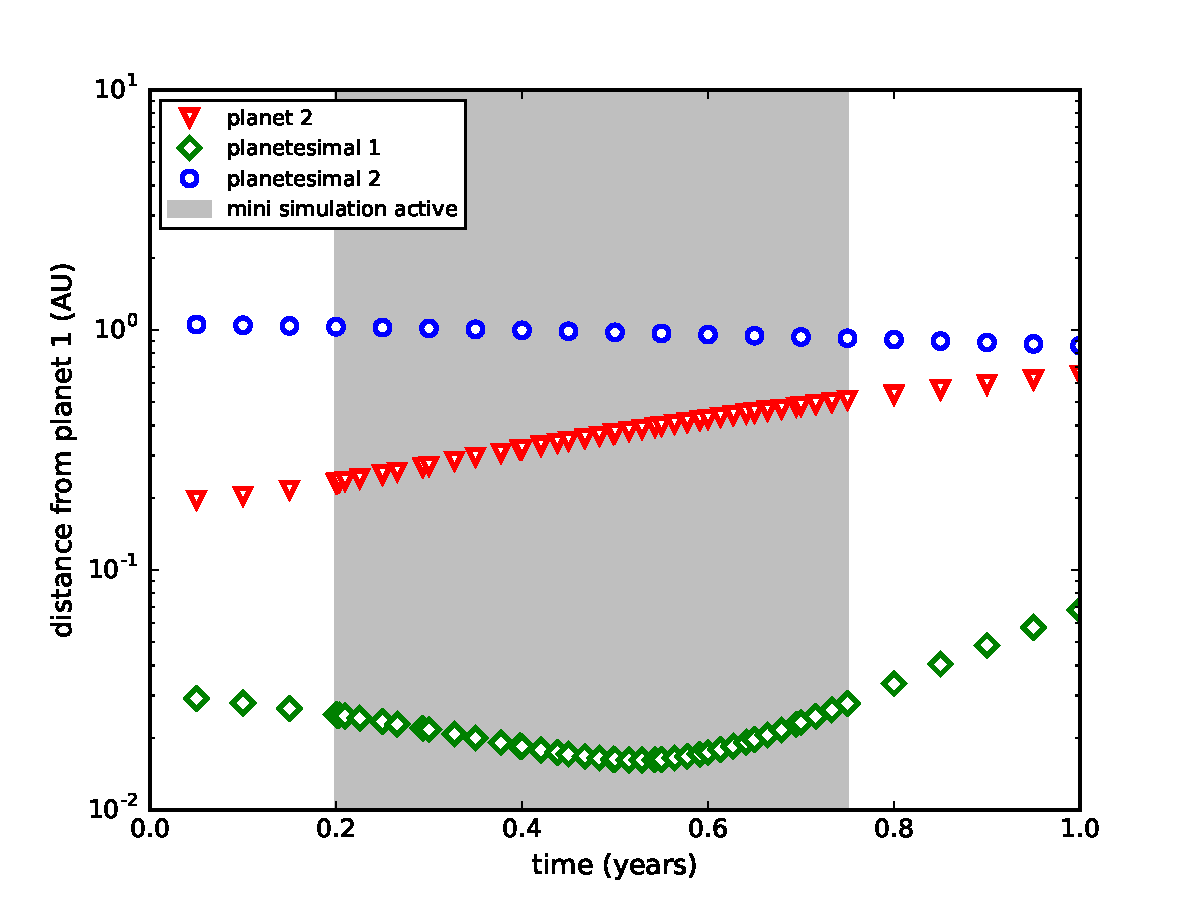
\includegraphics[scale=0.45]{chap4/images/CE_fig.pdf}}
\caption{
    A short simulation displaying the \hermes integrator for a 2~planet, 2~planetesimal system orbiting a central star. 
When active, the mini simulation takes many sub-timesteps for each $dt$ and integrates planets~1, 2~and planetesimal~1 during the close encounter between planet~1 and planetesimal~1. 
 }
\label{fig:CE_fig}
\end{figure}

We briefly discuss the speed of the algorithm.
If no particles are integrated with \ias, then the speed is effectively that of \whfast with a small overhead due to collision checks.
If all particles are integrated with \ias, then the speed is that of a simulation running only \ias, again with a small and in general negligible overhead due to collision checks. 
Consider a typical simulation of multiple active particles undergoing planetesimal migration from a large number of semi-active particles with a reasonable $\HSF$ value.
As the number of semi-active particles is increased, the ratio of the number of particles in the mini simulation, $N_{\rm mini}$, to the number of particles in the global simulation, $N_{\rm global}$, approaches a constant. 
In this limit the elapsed simulation time is linearly proportional to the number of semi-active particles in the simulation.

%%%%%%%%%%%%%%%%%%%%%%%%%%%%%%%%%%%%%%%%%%%%%%%%%%%
\subsection{Perturbative Forces in the Mini Simulation}
\label{sec:add}
One must carefully treat the forces perturbing the motions of active particles in the mini simulation. 
In the global simulation, active particles receive perturbative kicks from all semi-active particles, and it is important to reproduce these forces in the mini simulation, which only evolve a subset of particles. 
To further complicate this issue, the mini simulation takes numerous sub-timesteps for each global timestep.
In \hermes, we linearly interpolate the forces of all semi-active particles absent from the mini simulation using the initial and final values from the global simulation.
We find that interpolating the forces (rather than positions) leads to a significant speed gain without compromising noticeable accuracy.

One could argue that this process should be iterated -- the active particles will arrive at slightly different (and more accurate) final positions when integrated with the mini simulation, and thus the perturbative forces they would have induced on the semi-active particles in the global simulation would be slightly different too.
Thus if one wanted to improve the accuracy of the algorithm an iterative process could be constructed where the global and mini simulations take turns integrating for a timestep $dt$ making use of the updated positions from the previous iteration. 

However, as long as the semi-active particles have a much smaller mass than the active particles, we have found that this iterative process is unnecessary, allowing us to reduce both the computation time and algorithmic complexity.
We note that in our current non-iterative scheme, interpolating the forces between pairs of {\it active} particles introduces non-negligible numerical errors.
For that reason, all active particles are automatically added to the mini simulation during any close encounter, even if they are not involved in the close encounter themselves.

%%%%%%%%%%%%%%%%%%%%%%%%%%%%%%%%%%%%%%%%%%%%%%%%%%%
\subsection{Adaptive $\HSF$ Algorithm}
\label{sec:HSFop}
$\HSF$ and $dt$ are the most important parameters to consider when simulating a system with \hermes.
For a system free of close encounters, $dt$ alone determines the precision of the algorithm. 
However during close encounters $\HSF$ and $dt$ together determine the algorithm's precision (see Section~\ref{sec:Error}). 
Specifically, if a particle moves a distance $\sim \HSF r_H$ per timestep $dt$ the algorithm could miss a close encounter, introducing large errors into the simulation. 
In addition, an initial choice of $\HSF$ and $dt$ can become non-optimal if a system evolves significantly from its initial state. 

To aid the user in making the correct parameter choices, we have developed a simple algorithm that, given a timestep $dt$, conservatively estimates the smallest value of $\HSF$ under the condition that no close encounter is missed.
Although $\HSF$ and $dt$ both determine the precision of \hermes during a close encounter, we only optimize $\HSF$ since constantly changing $dt$ would result in non-negligible numerical errors for a symplectic integrator like \whfast.
We calculate the optimal $\HSF$ each iteration, ensuring that $\HSF$ adapts to an evolving system and guarantees that close encounters are continuously resolved.
The user is therefore only required to set the timestep $dt$ for a standard integration ($\SSF$ is set to a default value serving most purposes).
The full algorithm works as follows.

\begin{figure}
\centerline{\includegraphics[scale=0.6]{chap4/images/AutoHSF.pdf}}
\caption{Panel a. shows a regular orbit in 2D, while panel b. shows the construction of a ring by rotating the orbit's pericenter by $2\pi$.
 }
\label{fig:AutoHSF}
\end{figure}
For each body, we ignore the inclination, and marginalize over the phase and longitude of periapsis from $0$~to~$2\pi$.
As illustrated in Figure~\ref{fig:AutoHSF}, this smears out the orbit into a ring in the reference plane. 
Each ring has a maximum and minimum distance from the central object, $r_{\rm min}$ and $r_{\rm max}$.
We then check if any two interacting particles can possibly have a close encounter by comparing their $r_{\rm min}$ and $r_{\rm max}$ values.
If an intersection of two rings occurs, say for particles $i$ and $j$, we calculate their maximum relative velocity $\Delta v_{ij,\rm max}$ in the overlapping interval between the two particles.
We calculate $\Delta v_{ij,\rm max}$ as a simple overestimate rather than the true maximum in order to speed up the calculation.
As a result of ignoring the inclination and marginalizing over the phase and longitude of periastron, $\Delta v_{\rm max}$ can be calculated from just the semi-major axis and the eccentricity.
We note that we do not need to solve Kepler's equation in estimating $\Delta v_{\rm max}$.

We can then calculate $\HSF$ by taking the maximum over all interacting particle pairs (see Fig~\ref{fig:bodies}),
\begin{equation*}
\HSF = 4\;\underset{i,j}{\textrm{max}}\frac{ \Delta v_{ij,\rm max} dt}{r_{H, i} + r_{H,j}}.
\end{equation*}
The numerical constant $4$ ensures that two particles move at most one quarter of $\HSF (r_{H, i} + r_{H,j})$ in one timestep and therefore no close encounters are missed.

In practice, we also round up $\HSF$ to the nearest $1.25^x$ where $x$ is an integer to avoid continuous fluctuations in $\HSF$. 
By default, our adaptive $\HSF$ algorithm is enabled in \hermes.
Since the algorithm assumes particles move on approximately coplanar orbits, it may therefore fail at very high mutual inclinations.
We note that the above algorithm chooses the smallest value of $\HSF$ that captures all close encounters; however, small values of $\HSF$ introduce numerical errors when switching between integrators (see Section~\ref{sec:Error}).
Therefore, to avoid large errors we set a default lower limit of $\HSF=3$, which is close to the default close encounter boundary for \mercury and \symba.
The user can specify their own lower limit for $\HSF$ by setting {\sc \tt ri\_hermes.hill\_switch\_factor} at runtime. 

The adaptive $\HSF$ algorithm can be switched off by setting the variable {\sc \tt ri\_hermes.adaptive\_hill\_switch\_factor} to zero.
If the adaptive $\HSF$ algorithm is switched off, setting {\sc \tt ri\_hermes.hill\_switch\_factor} simply defines a constant value of $\HSF$ for the duration of the simulation (analogous to \mercury and \symba). 

We decided against devising a similar algorithm for $\SSF$ due to the additional difficulties that can arise. 
For example, an object in a circular orbit around a planet would be confused as a heliocentric orbit with a very high eccentricity, leading to large relative velocities and an excessive $\SSF$ value. 

%%%%%%%%%%%%%%%%%%%%%%%%%%%%%%%%%%%%%%%%%%%%%%%%%%%
%%%%%%%%%%%%%%%%%%%%%%%%%%%%%%%%%%%%%%%%%%%%%%%%%%%
\section{Error}
\label{sec:Error}
Several terms contribute to the relative energy error of an integrator \citep[e.g.][]{Rein2015a}:
\begin{equation}
E = E_{\rm floor} + E_{\rm round}  + E_{\rm bias} + E_{\rm scheme}.
\label{eq:error}
\end{equation}

$E_{\rm floor}$ is a constant due to the inability to represent numbers with arbitrary precision on a computer.  
Here we work exclusively in IEEE754 double floating point precision and thus have $E_{\rm floor}\sim 10^{-16}$. 

$E_{\rm round}$ arises when a computation is performed on two floating point numbers. 
Almost all operations (addition, multiplication, square roots) lead to a roundoff error at the level of the machine precision.
The IEEE754 standard guarantees that the round-off error in consecutive floating point operations is random, thus leading to a $\propto t^{1/2}$ growth of $E_{\rm round}$ with time.

$E_{\rm bias}$ is the error from any biased operations and grows at least as $\propto t$.
Biased operations can originate from poor implementations\footnote{For example, the expression \texttt{x*(2./3.)} multiplies $x$ by a number that is consistently slightly too big or too small when represented in binary.  By contrast, the expression \texttt{2.*(x/3.)} multiplies and divides $x$ by numbers that are exactly representable in binary and is unbiased.} or from library functions that the IEEE754 standard does not guarantee will return unbiased results\footnote{For example, the standard library function \texttt{sqrt()} returns an unbiased result whereas \texttt{sin()} returns a biased result.} .

$E_{\rm scheme}$, the final term in Eq.~\ref{eq:error}, is the error introduced by the algorithm itself. 
Typically, this quantity is bound for symplectic integrators but grows linearly with time for non-symplectic integrators.

The important question is which error term dominates, and the answer will depend on the problem at hand.
For example, if a three-body system (star and two planets) is integrated with \ias, $E_{\rm scheme}^{ias} \approx 10^{-28}$ and the dominant error term will be $E_{\rm round}$, starting at $10^{-16}$ and growing as $t^{1/2}$ \citep[see][]{Rein2015a}. 
If we instead integrate the system with \whfast, the dominant error term will be $E_{\rm scheme}$, which is determined both by the mass ratio in the system and the timestep. 
For typical parameters $E^{WH}_{\rm scheme} \sim 10^{-9}$, and only for very long simulation times ($\sim 10^{14}$ timesteps) will the growth of $E_{\rm round}$ dominate over $E^{WH}_{\rm scheme}$.
For biased implementations, $E_{\rm bias}$ will dominate the error budget at earlier times.  

For typical simulations integrated with \hermes, $E_{\rm scheme}$ will dominate. 
The WH algorithm integrates a slightly different Hamiltonian from the true Hamiltonian described by the system, leading to an error that oscillates in a bounded manner as long as the integrated Hamiltonian remains constant.
However each time a particle is transferred to or from the global simulation (see Section~\ref{sec:Alg}), the WH-integrated Hamiltonian changes, and thus the error will change too.
For a typical WH integration, working in democratic heliocentric coordinates\footnote{Although Figures~\ref{fig:HSFdE}, \ref{fig:dtdE}, and \ref{fig:HSFratio} along with the results in Section~\ref{sec:Examples} are all performed using \hermes with \whfast in Jacobi coordinates, we derive the error using democratic heliocentric coordinates. This is because, a) it is much simpler to do, and b) as discussed in Section~\ref{sec:Future} we believe that \hermes with \whfast in heliocentric coordinates is ultimately a better choice. At the time of this thesis, the transition from \hermes with \whfast in Jacobi to heliocentric coordinates was underway. However, as shown in Figures~\ref{fig:HSFdE}, \ref{fig:dtdE} and \ref{fig:HSFratio} the error derived from democratic heliocentric coordinates (Equation~\ref{eq:Escheme}) agrees well with the numerical experiments performed with \whfast in Jacobi coordinates.}, $E_{\rm scheme}$ is \citep[e.g.][]{Saha1994,Wisdom2006}:
\begin{equation}
E_{\rm scheme}^{\rm WH} = \frac{dt^2}{12} \left \{ \left \{H_K, H_{\beta} \right \},  0.5H_K + H_{\beta} \right \} + O(dt^4)
\label{eq:WHerr}
\end{equation}
Here $H_K$ is the Keplerian Hamiltonian, $H_{\beta} = H_C + H_I$ is the summed momentum cross-term and interaction Hamiltonians, respectively, and \{\} are Poisson brackets (the quantities are explicitly defined for a test case with three particles below). 
For large $N$-body systems, Eq.~\ref{eq:WHerr} quickly becomes very difficult to evaluate analytically. 
However, we can gain some insight by applying Eq.~\ref{eq:WHerr} to a simple system. 

\begin{figure}
\centerline{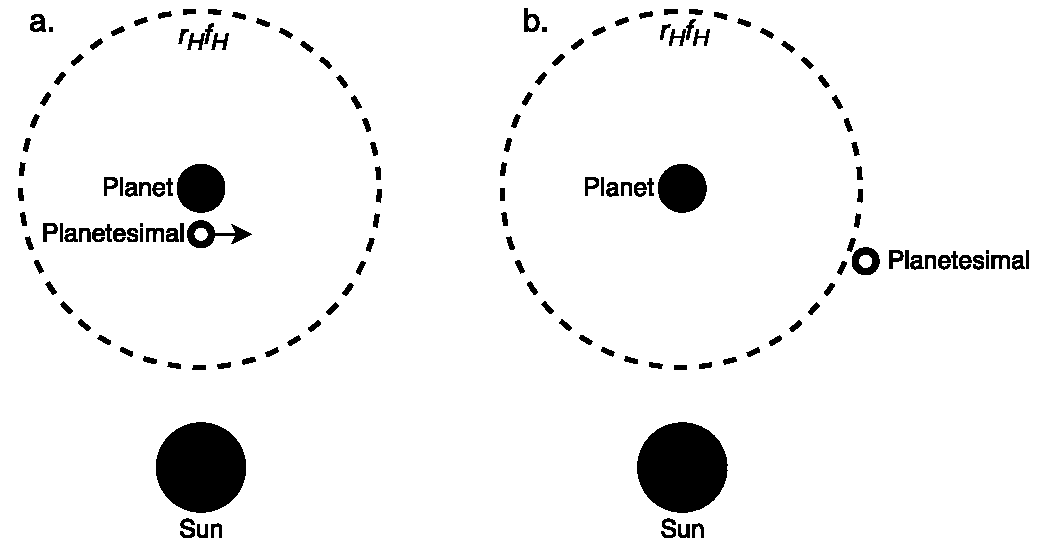
\includegraphics[scale=0.45]{chap4/images/R3B.pdf}}
\caption{Three body problem, in the reference frame of the planet. 
In a. the initial setup is shown, where the planetesimal starts near the planet, inside a sphere of radius $r_H\HSF$ and the entire system is integrated purely by \ias. 
Here the arrow indicates the initial direction of the planetesimal. 
In b. the planetesimal exits the sphere with radius $r_H\HSF$ and the system is integrated purely via \whfast, introducing a numerical error of $E_{\rm scheme}^{\rm WH}$.
}
\label{fig:R3B}
\end{figure}

We turn to a three body problem consisting of a star (active body), planet (active body) and planetesimal (semi-active body), shown in Figure~\ref{fig:R3B}.
The planetesimal is initially placed inside $\HSF$ with sufficient velocity such that the distance between the planet and planetesimal grows over time. 
While the planetesimal is inside $\HSF$ (panel a. in Fig.~\ref{fig:R3B}) the system is integrated to machine precision by \ias.
However once the planetesimal leaves $\HSF$ (panel b. in Fig.~\ref{fig:R3B}) the system switches to being integrated by \whfast, and an error of size $E_{\rm scheme}^{\rm WH}$ is introduced.

To estimate  $E_{\rm scheme}^{\rm WH}$, we start from the general Hamiltonian for an $N$-body system in democratic heliocentric coordinates:
\begin{equation*}
H = H_0 + H_K + H_C + H_I
\label{eq:Hbasic}
\end{equation*}
where $H_0$ is a constant describing the motion of the centre of mass along a straight line, and disappears when we evaluate Eq~\ref{eq:WHerr}. 
The remaining terms in Eq.~\ref{eq:Hbasic} take the form \citep{Duncan1998}:
\begin{align}
H_K &= \sum_{i=1}^{N-1} \frac{\bf{P}_i^2}{2m_i} - \sum_{i=1}^{N-1} \frac{Gm_0m_i}{|\bf{Q_i}|} \label{eq:H_K}\\
H_C &= \frac{1}{2m_0} \left|\sum_{i=1}^{N} \bf{P}_i \right|^2 \label{eq:H_C}\\
H_I &= -\sum_{i=1}^{N-1}\sum_{j=i+1}^{N} \frac{Gm_im_j}{|\bf{Q}_i - \bf{Q}_j|}\label{eq:H_I}
\end{align}
where the canonical coordinates $\bf{Q}$ and $\bf{P}$ are:
\begin{equation}
\bf{Q}_i = \begin{cases}
\bf{r}_i - \bf{r}_0 & \text{if } i \ne 0\\
\frac{1}{m_{\rm tot}}\sum_{j=0}^{N}m_jr_j & \text{if } i = 0\\
\end{cases}
\end{equation}
\begin{equation}
\bf{P}_i = \begin{cases}
\bf{p}_i - \frac{m_i}{m_{\rm tot}} \sum_{j=0}^{N} \bf{p}_j & \text{if } i \ne 0\\
\sum_{j=0}^{N} \bf{p}_j & \text{if } i = 0\\
\end{cases}
\end{equation}
Here $\bf{p}$, $\bf{r}$, $m$ are a particle's momentum, position and mass in any inertial frame respectively, while $G$ is the gravitational constant and $m_{\rm tot} =  \sum_{j=0}^{N} m_j$ is the total mass of the system.
$\bf{Q}_i$ are therefore heliocentric positions (with $\bf{Q}_0$ the centre of mass), while $\bf{P}_i$ are barycentric momenta (with $\bf{P}_0$ the momentum of the centre of mass).

We also further simplify the system to two dimensions by considering motion in a plane. 
One can then straightforwardly, albeit tediously, evaluate the Poisson bracket in Eq.~\ref{eq:WHerr} by plugging in Eqs.~\ref{eq:H_K}--\ref{eq:H_I} and taking derivatives with respect to all three particles. 
We make the further simplifying assumptions that $m_0 \gg m_2 \gg m_1$ and that $v_1 \approx v_2 \approx \sqrt{Gm_0/a}$, where $v$ denotes particle velocities and $a_2$ is the semi-major axis of the planet.
In addition, after solving Eq.~\ref{eq:WHerr} we set the distance of the planetesimal from the planet to $r_{H}\HSF$, where $r_{H}$ is the Hill radius of the planet. 
This is true at the moment the integration method is switched.
We are then left with a single dominating term,
\begin{equation}
\begin{split}
E_{\rm scheme}^{\hermes} \approx \frac{dt^2}{12} \frac{G^2 m_0m_1m_2}{a_2(r_{H}\HSF)^3},
\label{eq:Escheme}
\end{split}
\end{equation}
where we have ignored numerical constants of order unity.
An IPython notebook with a computer derivation is available at \url{https://github.com/silburt/hermes_ipython}.

\begin{figure}
\centerline{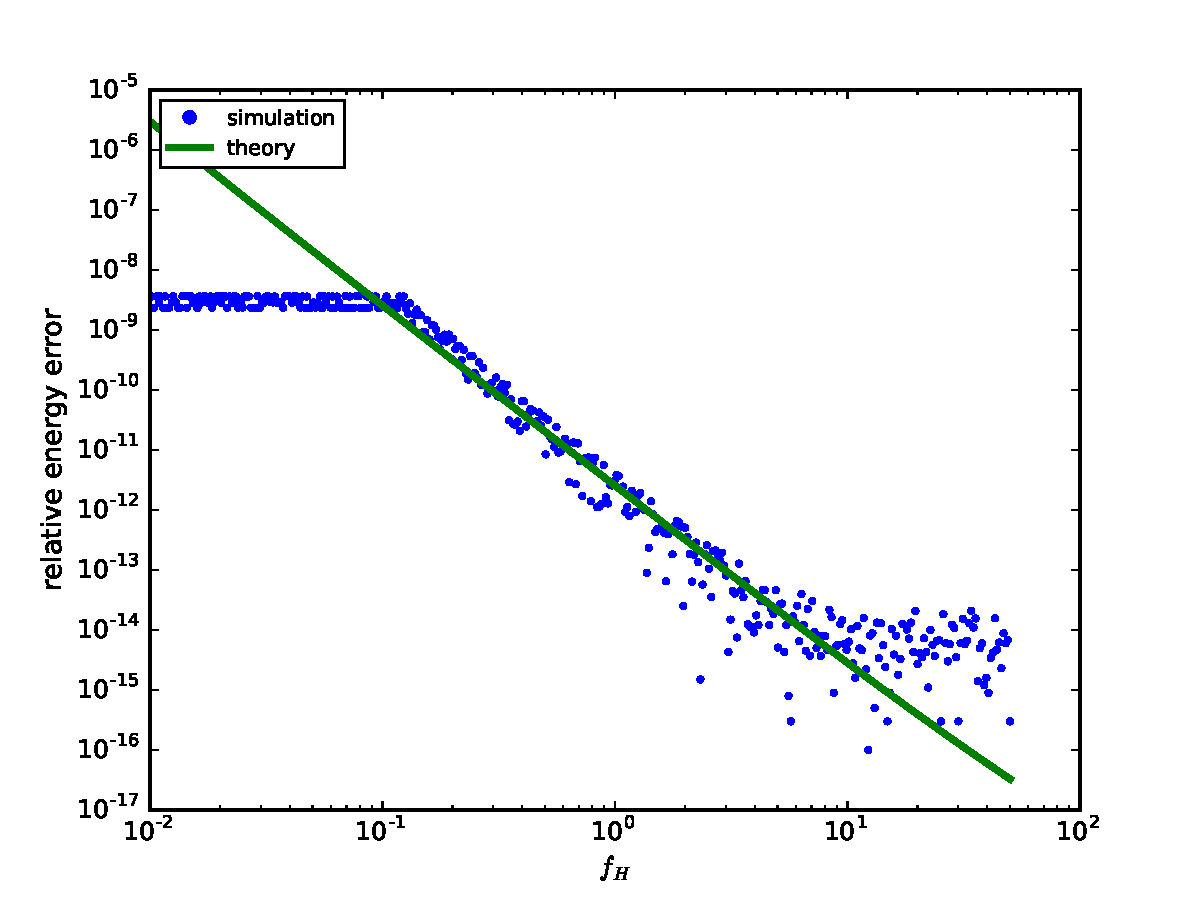
\includegraphics[scale=0.45]{chap4/images/HSR_v_dE.pdf}}
\caption{Final relative energy error as a function of $\HSF$ for a star-planet-planetesimal system. 
Blue dots are numerical simulations, the green curve is the theoretical prediction of Eq.~\ref{eq:Escheme}.
 }
\label{fig:HSFdE}
\end{figure}
We compare our theoretical predictions in Eq.~\ref{eq:Escheme} to numerical tests in Figures \ref{fig:HSFdE} and \ref{fig:dtdE}.
Our numerical setup consists of a star with mass $1M_\odot$, a Neptune mass planet on a circular orbit at $1$~AU, and a planetesimal with mass $10^{-8}M_\odot$ placed at $0.001$~AU from the planet.
To marginalize over the phase of the encounter when sampling the energy error, the initial position of the planetesimal is randomized for each realization.
In addition, the planetesimal is given a small kick equal to the escape velocity of the planet to ensure that the planetesimal-planet distance increases with time.
Each realization is simulated for 7 years.
When varying the timestep in Fig.~\ref{fig:dtdE} we use a constant $\HSF = 6$, and when varying $\HSF$ in Fig.~\ref{fig:HSFdE} we use a constant timestep of $dt = 0.058$~days.

In Figure~\ref{fig:HSFdE} one can see that the numerical tests agree with the theoretical predictions of Eq.~\ref{eq:Escheme}.
In addition, one can see the two extreme regimes on each end of the figure.
For particles starting outside the $r_H\HSF$ boundary the integrator always uses \whfast (like panel b. of Fig.~\ref{fig:R3B}), while for particles inside the $r_H \HSF$ boundary the simulation uses \ias (like panel a. of Fig.~\ref{fig:R3B}).
In Figure~\ref{fig:dtdE} one can see that the relative energy error is proportional to $dt^2$, again matching the predictions of Eq.~\ref{eq:Escheme}.
For both Fig.~\ref{fig:HSFdE} and Fig.~\ref{fig:dtdE}, we have not performed any kind of fit, we simply over-plotted Eq.~\ref{eq:Escheme} with the data from our numerical experiments. 
We have performed other suites of simulations testing how the energy error scales with all other relevant quantities (semi-major axis, planetesimal mass, planet mass, stellar mass) and find Eq.~\ref{eq:Escheme} in good agreement.
An IPython notebook for these experiments (including tests of the other relevant quantities) is available at \url{https://github.com/silburt/hermes_ipython}.

\begin{figure}
\centerline{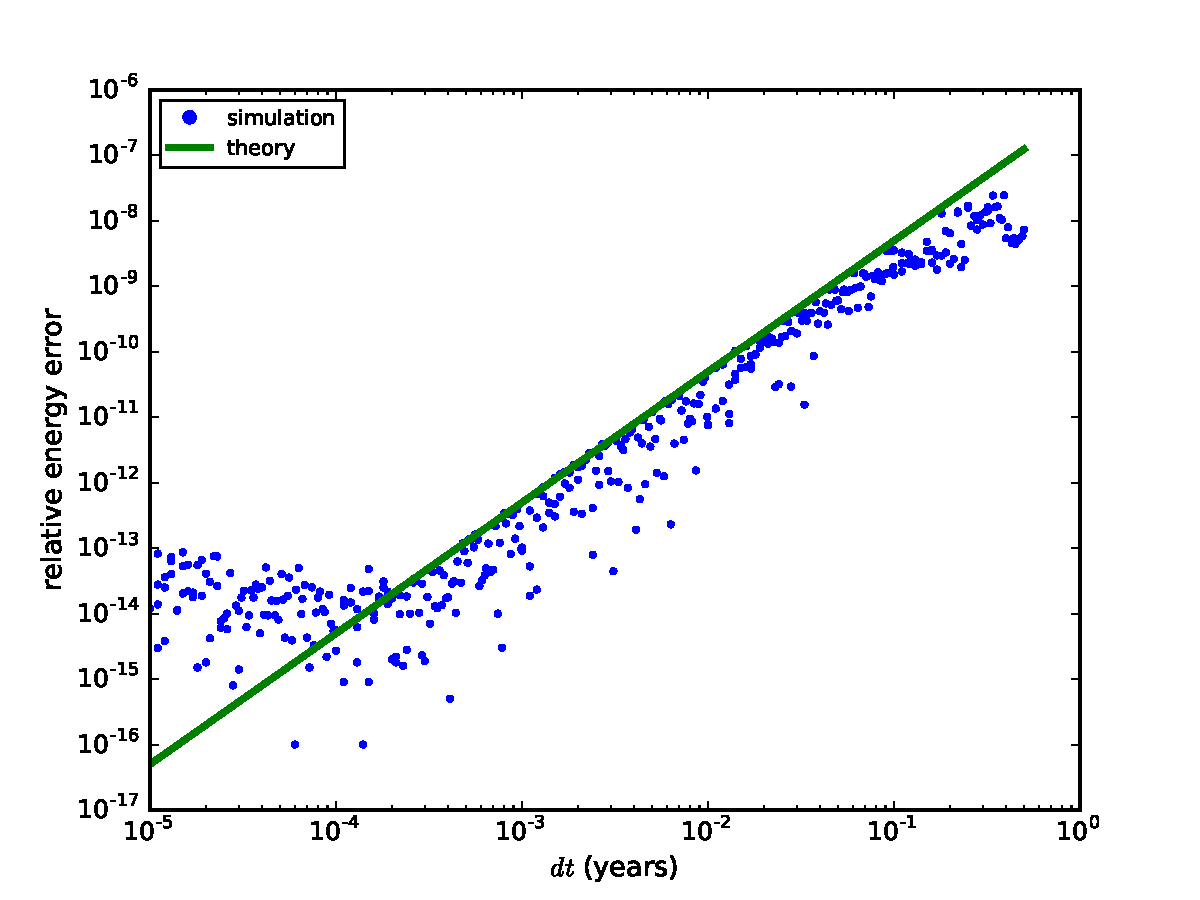
\includegraphics[scale=0.45]{chap4/images/dt_v_dE.pdf}}
\caption{Final energy error as a function of $dt$ for a star-planet-planetesimal system. 
Blue dots are numerical simulations, the green curve is the theoretical prediction of Eq.~\ref{eq:Escheme}.
 }
\label{fig:dtdE}
\end{figure}

We now extend the characterization of the error to a more realistic case with $N$ particles.
We refer to the total relative energy error for an integration as $E_{\rm scheme,tot}^{\hermes}$.
Since an error of size $E_{\rm scheme}^{\hermes}$ is introduced each time a particle leaves/enters the global simulation, the total errors should be related to the number of close encounters, $N_{\rm CE}$.
In the ideal case where the integrator is unbiased, the error $E_{\rm scheme}^{\hermes}$ introduced by each close encounter is random, and $E_{\rm scheme,tot}^{\hermes}$ will grow as a $N_{\rm CE}^{1/2}$ random walk.
However, if \hermes is biased (i.e. $E_{\rm scheme}^{\hermes}$ is not random), then $E_{\rm scheme,tot}^{\hermes}$ will grow faster than $N_{\rm CE}^{1/2}$. 

Assuming the unbiased case, $E_{\rm scheme,tot}^{\hermes}$ is equal to:
\begin{equation}
E_{\rm scheme,tot}^{\hermes} = K \cdot E_{\rm scheme}^{\hermes}  \cdot  \sqrt{N_{\rm CE}}
\label{eq:Etot}
\end{equation}
where $K$ is a constant of proportionality. 
We test Eq.~\ref{eq:Etot} against numerical tests for a Solar mass star, a Neptune mass planet on a circular orbit at $1$~AU, and a disk of 200 planetesimals located between $0.98 - 1.02$~AU.
The initial inclinations and eccentricities of the planetesimals in the disk are set to 0, while the argument of perihelion and true anomaly are drawn from a uniform distribution.
In addition, for these simulations we set $\HSF = 6$ and $dt = 0.015$ years. 
We performed numerous integrations, integrating each realization for a randomly chosen number of orbital periods between 10-1000, yielding different numbers of close encounters.

\begin{figure}
\centerline{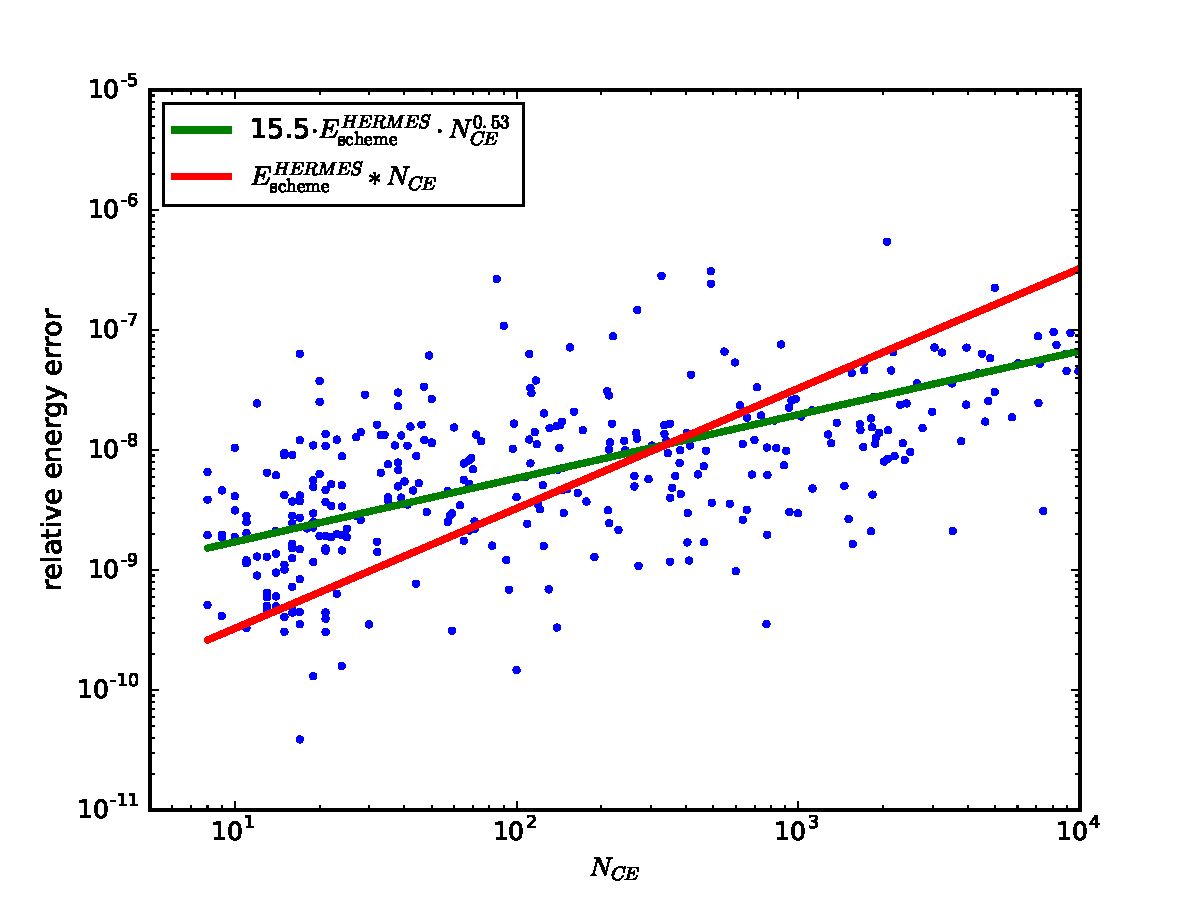
\includegraphics[scale=0.45]{chap4/images/CEvdE.pdf}}
\caption{Final relative energy error as a function of the number of close encounters, for a system composed of a star, planet and 200 planetesimals. 
Blue dots are numerical simulations, the green line is our unbiased theoretical prediction of Eq.~\ref{eq:Etot} with $K = 15$, while the red line is the biased theoretical prediction.
 }
\label{fig:HSFratio}
\end{figure}

The results are shown in Figure~\ref{fig:HSFratio}, the x-axis showing the number of close encounters during a simulation and the y-axis showing the final relative energy error for each simulation.
We fit a power-law distribution to the data using Python's Scipy Optimize Curve Fit package \citep{Scipy2016}, displayed as a green line in Fig.~\ref{fig:HSFratio}. 
The resulting fit is $E_{\rm scheme,tot}^{\hermes}= 15.5 \cdot E_{\rm scheme}^{\hermes} \cdot N_{\rm CE}^{0.53}$, so the energy growth is well approximated by Eq.~\ref{eq:Etot}. 
For reference, we plot the biased prediction of $E_{\rm scheme,tot}^{\hermes} \propto N_{\rm CE}$ as a red line.
We conclude that \hermes is unbiased for this setup.
Thus, Eq.~\ref{eq:Etot} provides an intuitive way of understanding how the error of \hermes grows without having to analytically solve Eq.~\ref{eq:WHerr} in three dimensions for $N$ particles. 

The results from Fig.~\ref{fig:HSFratio} did not allow for physical collisions between particles. When physical collision are enabled a systematic bias can be introduced. 

To see why, note that for each close encounter two contributions to the energy error arise according to Eq.~\ref{eq:Escheme}; one when the particles are transferred from the global to the mini simulation (i.e. the ingress of the close encounter) and one when the particles are transferred back from the mini to the global simulation (i.e. the egress of the close encounter).
The precise energy change depends on the specific properties of the system (phases of the orbits, angles of approach, etc.), and typically the energy changes associated with the ingress and egress of the close encounter are anticorrelated. 
As a result, no appreciable energy error is introduced by close encounters, and the energy over the course of a simulation grows as expected according to Eq.~\ref{eq:Etot}.

However, when a physical collision occurs in \hermes,  the close encounter only has an ingress, resulting in a biased growth in the energy error. 
In practice this energy bias is orders of magnitude smaller than the physical energy lost during a collision, and therefore should not interfere with the longterm evolution of a system. 
We plan to study this issue in more detail in the future. 

\section{Examples}
\label{sec:Examples}
\hermes is well suited for a number of astrophysical problems, including planets embedded in planetesimal disks, high eccentricity comets, planet-planet scattering, star clusters orbiting a central potential, and more. 
Many example problems can be found at \url{https://github.com/hannorein/rebound/tree/master/ipython_examples}.
Below, we highlight just a few example problems that can be simulated with \hermes.

\subsection{Massive Outer Solar System}
Both \citet{Duncan1998} and \citet{Chambers1999} simulated the outer Solar System, but increased the masses of all planets by a factor of 50 to trigger close encounters between planets.
Analogous to \citet{Chambers1999} and \citet{Duncan1998} we use $\HSF=3$, $dt= 0.03$~yrs, and integrate the system for 1000 years. 

We perform a number of simulations of the massive outer Solar System, and find that the relative energy error stays bounded at~$\sim 10^{-7}$ for all simulations, matching the results of \citet{Chambers1999} and \citet{Duncan1998}. 

\subsection{Migration of a Planet in Planetesimal Disk \citep{Kirsh2009} }
Here we reproduce the results of \citet{Kirsh2009} for the migration of a single planet embedded in a planetesimal disk. 
In this study a 2.3$M_{\oplus}$ planet orbits a Solar mass star at $25$~AU, embedded in a disk of $\sim6\cdot10^4$~planetesimals. 
The planetesimal disk extends 10.5 AU on each side of the planet, each planetesimal has a mass 1/600th of the planet, and an overall surface density profile proportional to $a^{-1}$ is used.
The radii of all orbiting particles were determined assuming a constant density of $2~\rm{ g/cm^3}$.
The eccentricities and inclinations were drawn from a Rayleigh distribution, which is parameterized by the scale parameter $\sigma$.
For this experiment we use $\sigma_e = 0.01$, and $\sigma_i = 0.005$, where inclination is in radians.
The argument of periapse, true anomaly, and longitude of ascending node were all randomly drawn from uniform distributions over $[0, 2\pi]$.
Adopting the default settings of \citet{Kirsh2009}, we set \hermes to merge particles inelastically, set $dt=2$ years, $\HSF = 5$, $\SSF = 15$, and track the energy lost due to collisions or ejections. 
We also set {\sc \tt r->ri\_hermes.adaptive\_hill\_switch\_factor} = 1, activating the adaptive Hill switch routine (Section~\ref{sec:HSFop}).
An IPython notebook containing the code to run this example can be found at \url{https://github.com/silburt/hermes_ipython}.

We run 6 separate simulations, each for 70,000 years, and plot the results in Fig.~\ref{fig:Kirsh}.
The relevant comparison plot in \citet{Kirsh2009} is the lower right panel in Figure~3.
For all runs in both \citet{Kirsh2009} and our work the final position of the planet is between $18.5 < a < 20$ AU, and show similar evolution tracks throughout the simulation. 
The relative energy error over the course of all our simulations do not exceed $2\cdot10^{-7}$ after accounting for the energy lost in inelastic collisions. 

\begin{figure}
\centerline{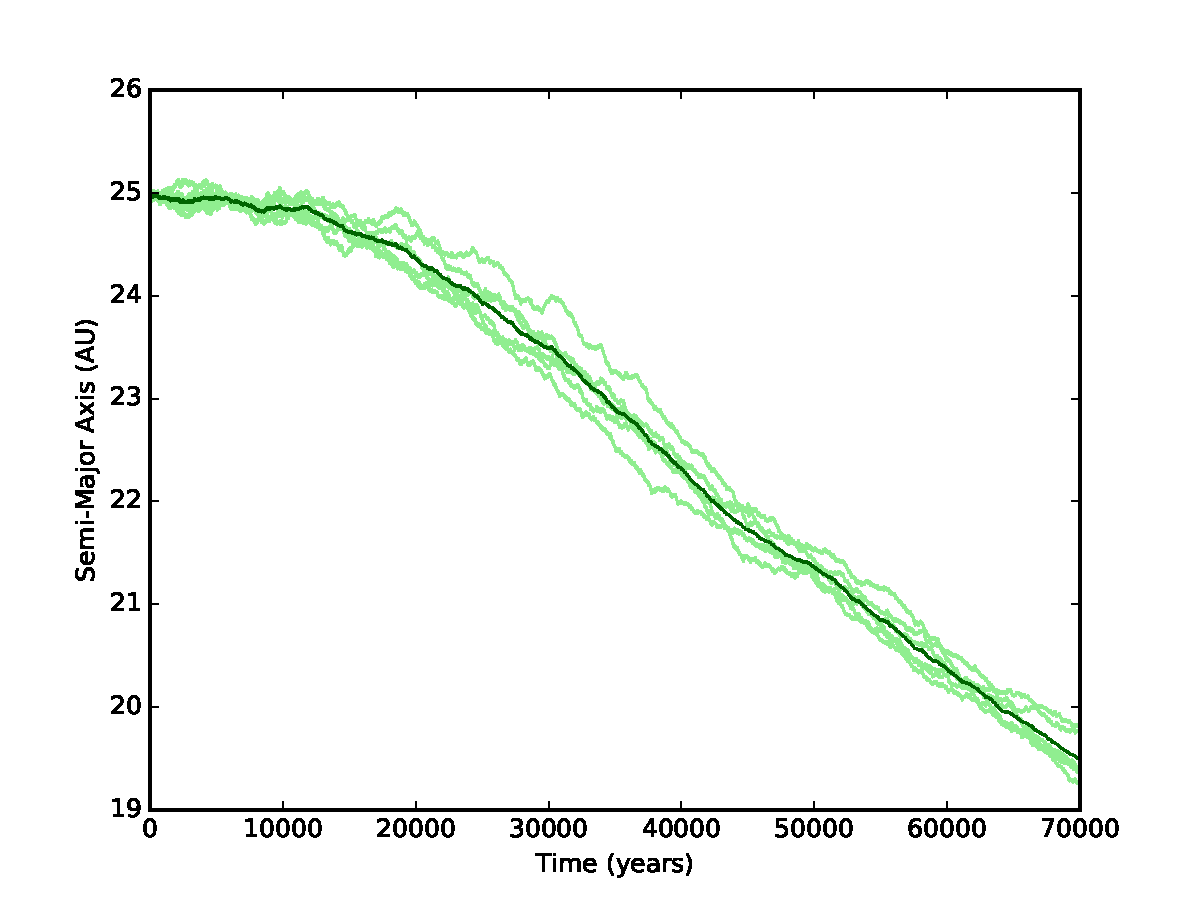
\includegraphics[scale=0.45]{chap4/images/Kirsh_avg_a.pdf}}
\caption{
Planet's semimajor axis vs. time, analogous to the numerical experiment in the lower right panel of Figure~3 from  \citet{Kirsh2009}. 
Light green lines represent individual runs, while the dark thicker green line represents the average of the individual runs. 
 }
\label{fig:Kirsh}
\end{figure}

\subsection{Comparison to \mercury and \symba -- Long Simulations}
Here we perform a set of long simulations and compare our results to \mercury and \symba.
These integrators are also capable of integrating complex $N$-body systems with close encounters, and also make use of semi-active particles.
The simulations for these tests contain a Solar-mass star, a Neptune-mass planet at $a=1$~AU and a disk of 100~semi-active planetesimals distributed according to a powerlaw between $0.8 - 1.2$~AU. 
The mass of each planetesimal is a third of a lunar mass, the eccentricities and inclinations are set to 0, and the argument of periapse, true anomaly, and longitude of ascending node were all randomly drawn from uniform distributions over $[0, 2\pi]$.
We set $dt = 0.01$, $\HSF = 3$, merge particles inelastically, and use our adaptive $\HSF$ routine (Section~\ref{sec:HSFop}). 
In addition, for all three integrators we track the energy lost due to inelastic collisions and ejections so that we can isolate the numerical energy error. 
We accomplish this by using the \texttt{eoffset} variable in \symba and \texttt{EN(3)} variable in \mercury, and calculate the relative energy error according to $(E_{i} + E_{\rm off} - E_{\rm 0})/E_{0}$, where $E_i$ is the total energy at iteration $i$, $E_0$ is the initial total energy and $E_{\rm off}$ is the energy lost due to collisions and ejections, i.e. \texttt{eoffset} in \symba and \texttt{EN(3)} in \mercury. 

We feed identical initial conditions to \symba, \mercury and \hermes, and evolve all simulations for 50 Myr. 
We run 6 simulations per integrator that differ only by the seed of the random number generator.
We average the relative energy error for these simulations to smooth out variations between individual runs.
The results are presented in Figure~\ref{fig:Np100test}.
The top panel displays the relative energy error with each integrator, while the bottom panel shows the elapsed time for each individual run.

\begin{figure}
\centerline{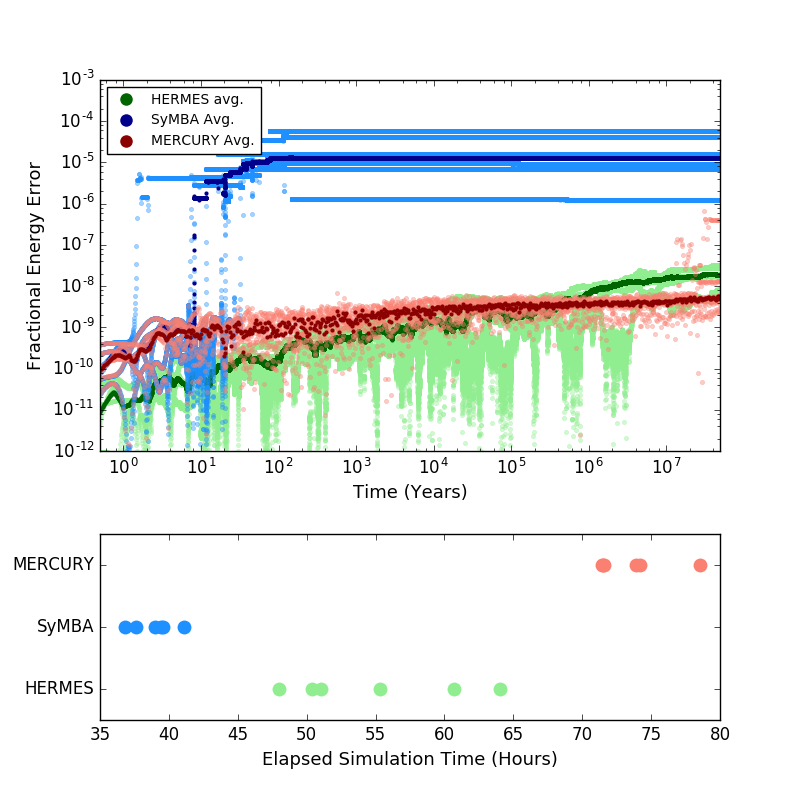
\includegraphics[scale=0.45]{chap4/images/energy_avg_FULL.png}}
\caption{A test of \hermes, \mercury and \symba for collections of 50Myr, 50 planetesimal runs. 
Top panel shows the relative energy error over time, with individual runs in lighter shades and averaged values in dark shades.
Bottom panel shows the elapsed simulation times of individual runs, using the same colour scheme as the top panel.
 }
\label{fig:Np100test}
\end{figure}

Looking at the top panel, \symba incurs significant energy jumps early in the simulation. 
We suspect these energy jumps are due to inadequately resolved close encounters, since the energy jumps are uncorrelated with particle collisions. 
We simulated runs using different combinations of {\sc \tt RHSCALE} and {\sc \tt RSHELL}, i.e. the parameters which define close encounter regions, but were unable to resolve these energy jumps. 
By the end of the simulation, \symba is orders of magnitude less accurate than \mercury and \hermes.

We see that \hermes initially has the lowest energy error, but grows faster than \mercury.  
The final energy error for an integration therefore depends on the particular problem (length of simulation, timestep, number and severity of close encounters etc.).
Furthermore, we find that some \mercury simulations undergo significant energy jumps, probably also due to very close encounters that are not properly resolved. 
Our adaptive $\HSF$ algorithm (Section~\ref{sec:HSFop}) protects against these situations from occurring, and for a properly chosen $\HSF$ and $dt$ combination we find the energy growth of \hermes to be well behaved. 

The bottom panel shows that for these simulations \hermes is slower than \symba but faster than \mercury. 
We see that \hermes exhibits a larger variance in elapsed simulation times than \mercury and \symba. 
This is because when the adaptive $\HSF$ routine is engaged, $\HSF$ can be enlarged considerably during severe encounters, slowing down the integrator. 
In summary, these simulations show that \hermes provides a good balance between speed and accuracy.

\section{Conclusion}
\label{sec:Conclusion}
In this Chapter we have presented \hermes, a hybrid integrator capable of integrating close encounters and collisions. 
\hermes integrator is composed of two parts, a global simulation which contains all particles and a mini simulation which contains all active particles (e.g. stars and planets) plus any semi-active/test particles (e.g., planetesimals) involved in a close encounter.
The global simulation is integrated with \whfast while the mini simulation is integrated with \ias.
Comparing \hermes to the openly available \mercury and \symba we find that \hermes provides a good balance between accuracy and speed.

\hermes takes a more direct approach when integrating close encounters over other methods.
However this has enabled us to characterize the error of \hermes, and we find that the switching error from a single close encounter is well described by Eq.~\ref{eq:Escheme}, which we calculate from first principles.
The total energy error of \hermes for an $N$-body simulation is well described by a random walk, (see Eq.~\ref{eq:Etot}) with the step size being the switching error.

We have also developed an adaptive algorithm that chooses the optimal Hill switch factor, $\HSF$, which governs the size of the close encounter region surrounding each particle.
This frees the user from optimizing integrator parameters for typical cases. 
Finally, we have introduced a number of new features in \reb, including semi-active particles (see Fig.~\ref{fig:bodies}) and inelastic collisions.

We have showcased a number of problems well-suited for \hermes, and compared our integrator's performance to similar integrators in the literature. 
In particular, we integrated the outer Solar System with planetary masses increased by a factor of 50, and we simulated a planet migrating through a disk of planetesimals, both in the limit of many planetesimals ($\sim 10^5$) and short times ($\sim 10^3$ orbits), and few planetesimals (100) and long times ($\sim 10^8$ orbits).
Many more types of problems are possible with \hermes, and additional examples can be found at {\sc \tt https://github.com/hannorein/rebound}.
